% !TEX program = xelatex
\documentclass[UTF8,a4paper,10pt]{ctexart}
\usepackage[margin=2.05cm]{geometry}
\usepackage{graphicx}
\usepackage{booktabs}
\usepackage{tabularx}
\usepackage{array}
\usepackage{amsmath}
\usepackage{xcolor}
\usepackage{hyperref}
\usepackage{caption}
\usepackage{float}
\usepackage[numbers,sort&compress]{natbib}
\graphicspath{{figures/}}
% Generated by scripts/generate_dataset_figures.py.
\newcommand{\DatasetSceneCount}{10}
\newcommand{\DatasetTiffCount}{60}
\newcommand{\DatasetUsablePatchCount}{1800}
\newcommand{\DatasetPrivacyExcludedCount}{25}
\newcommand{\DatasetFixedTrainCount}{1141}
\newcommand{\DatasetFixedValidationCount}{270}
\newcommand{\DatasetFixedTestCount}{389}
\newcommand{\DatasetTaskFileCount}{14400}
\newcommand{\DatasetRawFileCount}{1281}
\newcommand{\DatasetSourcePositionCount}{140}
\newcommand{\DatasetRgbFrameCount}{581}
\newcommand{\DatasetSwirFrameCount}{700}
\newcommand{\DatasetPoseEdgeCount}{591}
\newcommand{\DatasetOutputScale}{3.2}
\newcommand{\DatasetAcquisitionDateMin}{2025-04-29}
\newcommand{\DatasetAcquisitionDateMax}{2025-11-28}
\newcommand{\DatasetCoverageMin}{0.712}
\newcommand{\DatasetCoverageMax}{0.902}
\newcommand{\DatasetCoverageMean}{0.841}
\newcommand{\DatasetBuildSecondsMin}{48.6}
\newcommand{\DatasetBuildSecondsMax}{908.1}
\newcommand{\DatasetRedactedSceneUsablePatchCount}{131}
\newcommand{\RegHoldoutMinPx}{3.56}
\newcommand{\RegHoldoutMedianPx}{5.73}
\newcommand{\RegHoldoutMeanPx}{6.06}
\newcommand{\RegHoldoutMaxPx}{9.23}
\newcommand{\RegCornerMinPx}{1.56}
\newcommand{\RegCornerMedianPx}{3.03}
\newcommand{\RegCornerMeanPx}{5.70}
\newcommand{\RegCornerMaxPx}{27.78}
\newcommand{\RegCornerWorstScene}{C5}
\newcommand{\RegCornerRunnerUpPx}{8.60}
\newcommand{\RegCornerOutlierRatio}{3.2}
\newcommand{\RegCornerOtherMeanPx}{3.24}
\newcommand{\RegCornerGateMinPx}{25.6}
\newcommand{\RegCornerGateMaxPx}{76.3}
\newcommand{\IntraSwirMinPx}{3.19}
\newcommand{\IntraSwirMeanPx}{4.74}
\newcommand{\IntraSwirMaxPx}{6.25}
\newcommand{\IntraSwirGatePx}{8}

\hypersetup{colorlinks=true,linkcolor=black,citecolor=black,urlcolor=blue}
\setlength{\parindent}{2em}
\setlength{\parskip}{0.25em}
\setlength{\emergencystretch}{2em}
\captionsetup{font=small,labelfont=bf}
\newcommand{\pending}[1]{\textcolor{red}{[待补：#1]}}

\title{\textbf{面向跨光谱图像生成的场景级RGB与五波段短波红外配对数据集}}
\author{杜虎$^{1,2,*}$，刘晓$^{2,3,\dagger}$，杜丽丽$^{2,3}$，宋波$^{2,3}$，孙晓兵$^{2,3}$\\[0.35em]
\small $^{1}$中国科学技术大学，合肥 230026，中国\\
\small $^{2}$中国科学院合肥物质科学研究院，合肥 230031，中国\\
\small $^{3}$中国科学院安徽光学精密机械研究所光学定标与表征重点实验室，合肥 230031，中国\\[0.25em]
\small $^{*}$通讯邮箱：\href{mailto:2542497213@qq.com}{2542497213@qq.com}（杜虎）；$^{\dagger}$\href{mailto:liux@aiofm.ac.cn}{liux@aiofm.ac.cn}（刘晓）\\
\small ORCID（杜虎）：\href{https://orcid.org/0009-0006-1742-2455}{0009-0006-1742-2455}}
\date{}

\begin{document}\maketitle
\pending{2026-09-24协议同步稿，非最终投稿版。人工验收与新协议正式实验未完成；旧69次/三种子结果仅留在历史备份。}
\begin{abstract}RGB与短波红外（SWIR）配对影像的可靠复用依赖明确的光谱定义、空间对应关系与评价单位。M-SWIR-RGB包含十个不同物理地点的十个场景拼接图，由140个采集视野、1281个原始文件（581幅RGB、700幅SWIR）构建。每个地点提供RGB与五个名义SWIR波段，共60幅八位TIFF。五波段采用时分采集，未进行辐射定标。本文记录源文件身份、几何变换、辐射处理和隐私排除。当前验证协议将六模态独立检查点、盲法重复标注、内容区域与局部质量区域结合，并采用地点隔离的五折、五种子评价；最终掩膜与训练池将在模型评价前冻结。本同步稿陈述当前协议，人工独立验证统计和正式基准结果仍待完成，不将历史基准数值作为当前结果。\end{abstract}
\section{概要}
本数据描述稿以原始观察、地点身份、处理来源、独立人工证据和可复用评价协议为主要贡献，数据文档化遵循数据表与FAIR原则的实践\cite{gebru2021,wilkinson2016}。可见光--红外与多光谱配对资源已支持语义分割、检测与跨模态匹配\cite{ha2017,hwang2015,jia2021,razakarivony2016}；跨光谱着色与合成方法依赖此类配对\cite{levin2004colorization,zhang2016colorful,chen2025}；SWIR在材质判别与恶劣条件感知中的价值亦有报道\cite{song2024,bijelic2020fog}。数据用于跨光谱生成与多模态研究，不以提出新模型为目标。同平台既有工作需在投稿前完成原图重叠与新增内容披露。
\begin{figure}[htbp]\centering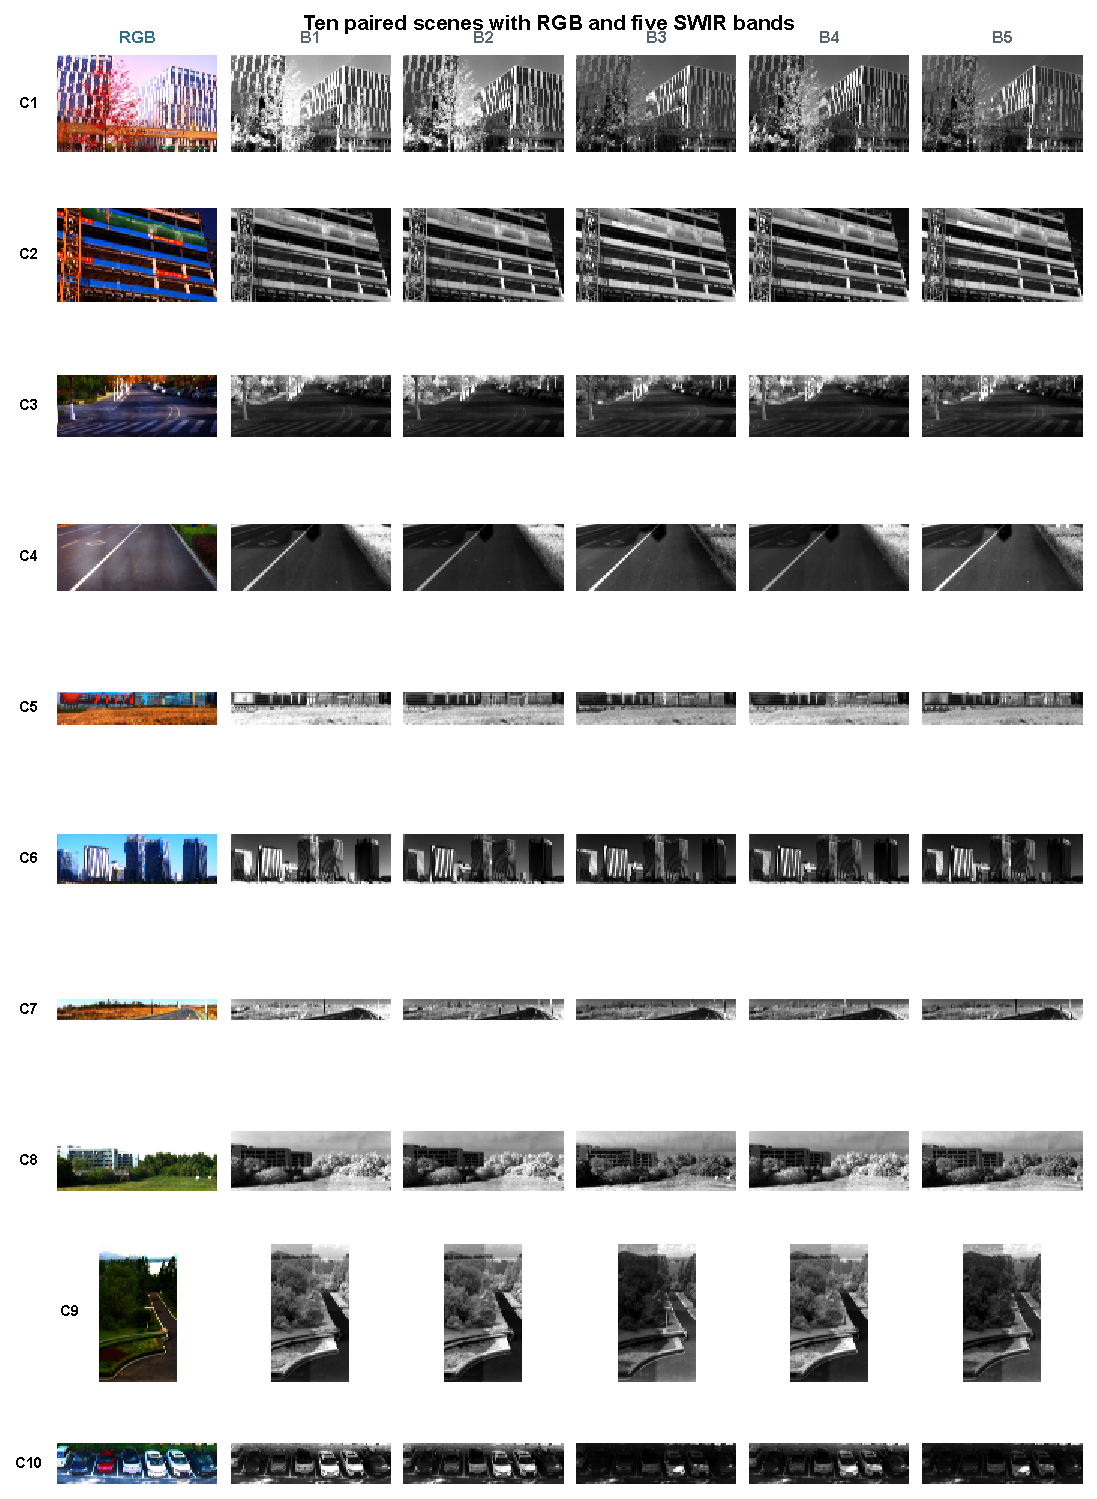
\includegraphics[width=\textwidth]{fig1_scene_modality_overview.pdf}\caption{六模态成图总览。仅用于显示的全局分位拉伸不参与评价；本图不证明局部配准精度。}\label{fig:overview-zh}\end{figure}
\begin{table}[htbp]
\centering
\caption{与已有配对数据资源的结构性比较。其他资源的条目取自其公开描述；``n.r.''表示被引文献未报告，本文未独立核实。}
\label{tab:related-zh}
\small
\begin{tabularx}{\textwidth}{@{}p{0.13\textwidth}p{0.17\textwidth}p{0.20\textwidth}p{0.20\textwidth}X@{}}
\toprule
资源 & 场景域 & 光谱内容 & 配对机制 & 组织方式与划分\\
\midrule
RASMD \cite{jin2026} & 驾驶，城市/郊区，晴、阴、雨、雪 & RGB加一个宽带SWIR通道（1000--1700\,nm） & 两台独立相机，事后SIFT单应与RANSAC & 每模态$10^5$帧；帧级划分（训练1432、测试956）\\
AVIID \cite{aviid2023} & 航拍，车辆目标 & 可见光与红外图块对 & 分开航拍获取 & 993、1090与1280对，$434\times434$或$512\times512$；图块级\\
DeepSWIR \cite{rout2019} & 卫星多传感器 & 由绿、红、近红外与粗分辨率SWIR合成的SWIR波段 & 跨传感器配准，5与24\,m GSD & n.r.\\
同平台早期发布 \cite{chen2026threeband,chen2026thesis} & 地面场景，四类 & 三个SWIR波段（B1、B2、B4） & 共孔径平台，先拼接后滑动窗口 & 4000对图块；随机4:1训练/测试划分\\
M-SWIR-RGB（本发布） & 地面场景，四类，十个不同地点 & RGB加五个实测SWIR波段 & 共孔径二向色平台；逐场景特征位姿图 & \DatasetSceneCount{}个场景；新池待冻结；场景隔离的训练/验证/测试\\
\bottomrule
\end{tabularx}
\end{table}
\section{方法}
\paragraph{证据边界}以下平台与能量表沿用已引用的既有平台文献；能量值是模型计算，不是本数据集的实测光谱响应，材料可分性推断不构成本稿新增实验结果。\pending{作者核对本批采集设置与既有文献一致性。}
\subsection{采集平台}
配对采集采用共孔径二向色分光平台，而非两台各自独立瞄准的相机。景物辐射先经前置物镜，到达以45$^{\circ}$放置的分光镜：波长小于900\,nm的部分被反射进入垂直方向的可见光支路，波长大于900\,nm的部分透射进入水平方向的SWIR支路。由于两个传感器通过同一入射光瞳观测场景，双相机并排方案中的视差在光路层面即被消除，目标的相对像面位置不随远近变化。残余失配仍来自两支路像元间距、靶面尺寸与后光路镜头畸变的差异，因此几何配准仍是必需的处理步骤\cite{zitova2003}。

可见光支路搭载PCO panda 4.2 sCMOS相机（$2048\times2048$像素，450--680\,nm），SWIR支路搭载Xenics Bobcat 640相机，其InGaAs焦平面为$640\times512$像素、响应范围900--1700\,nm\cite{rogalski2003}。五个窄带干涉滤光片安装于SWIR传感器前端的电动滤光片轮（Thorlabs FW102C）。每个位置由同一段采集软件序列驱动滤光片轮换位与两台相机的曝光，因此同一位置的RGB与SWIR由同一序列触发。但SWIR通道本质上是分时而非快照式：同一位置的五个波段是对近似静态场景的连续曝光，而不是五次同时测量。曝光间隔内发生的任何场景变化都会成为波段间不一致，且无法由任何配准步骤消除（表~\ref{tab:hardware-zh}）。可见光与短波红外多光谱成像的系统级设计另见\cite{yu2024}；该平台的详细设计见文献\cite{chen2026thesis}。

\begin{table}[htbp]
\centering
\caption{采集平台组成。}
\label{tab:hardware-zh}
\small
\begin{tabularx}{\textwidth}{@{}p{0.20\textwidth}X@{}}
\toprule
组件 & 参数\\
\midrule
分光结构 & 共入射光瞳；45$^{\circ}$二向色分光镜，$<$900\,nm反射至可见光支路，$>$900\,nm透射至SWIR支路\\
可见光相机 & PCO panda 4.2 sCMOS，$2048\times2048$像素，450--680\,nm\\
短波红外相机 & Xenics Bobcat 640，InGaAs焦平面，$640\times512$像素，900--1700\,nm\\
滤光片轮 & Thorlabs FW102C，电动，五个位置，分时切换波段\\
滤光片 & Edmund Optics窄带干涉滤光片，带宽50\,nm（表~\ref{tab:bands-zh}）\\
触发方式 & 每个位置由一段软件序列驱动滤光片轮换位与两路曝光\\
\bottomrule
\end{tabularx}
\end{table}

\subsection{光谱波段定义}
五个通带在数据采集之前即已确定，依据是在InGaAs响应范围内建立的有效能量积分模型：
\begin{equation}
E_{[\lambda_1,\lambda_2]}=\int_{\lambda_1}^{\lambda_2}E_{\mathrm{sun}}(\lambda)\,\tau_{\mathrm{atm}}(\lambda)\,\eta_{\mathrm{QE}}(\lambda)\,\mathrm{d}\lambda ,
\label{eq:energy-zh}
\end{equation}
其中$E_{\mathrm{sun}}$为ASTM G173标准太阳光谱辐照度\cite{astmg173}，$\tau_{\mathrm{atm}}$为在中纬度冬季大气模型与乡村型气溶胶模型参数下由MODTRAN仿真得到的大气透过率\cite{berk2014modtran}，$\eta_{\mathrm{QE}}$为InGaAs探测器量子效率。将900--1700\,nm以100\,nm为区间积分统计，可区分出三个高能量、低方差窗口（1000--1100、1200--1300与1500--1700\,nm）以及两个受水汽强吸收\cite{mccartney1976,bohren1983}主导的区间；后者的能量均值分别降至0.065与0.028，因而不具备常规成像价值并被排除（表~\ref{tab:energy-zh}）。能量最高的窗口被拆分为两个相邻的50\,nm通道，原因是该窗口内植被与裸土的反射率差异较小，在信号最强处加密光谱采样可提升材质可分性；典型地物的区分能力依据NASA AVIRIS光谱库评估\cite{chen2026thesis}。波段选择与波段数--性能权衡的通用方法背景见\cite{chavez1982oif,bsnets2020,hughes1968}。

该定义有两点限制必须明确说明，因为它们约束数据的复用方式。其一，表中通道为滤光片的名义规格，并非系统级实测结果：装配后的光学系统、滤光片与探测器链路的相对光谱响应从未被定标，因此实际带内形状与干涉滤光片的带外泄漏在发布数据中没有任何记录。其二，全流程未做任何辐射定标。所有发布的像素值均为八位数字量，波段间比值应理解为仪器相关量，而非地表反射率\cite{schott2007}。

\begin{table}[htbp]
\centering
\caption{SWIR通道定义。通道为滤光片名义规格；装配系统的端到端相对光谱响应未实测。}
\label{tab:bands-zh}
\small
\begin{tabular}{@{}lllll@{}}
\toprule
通道 & 名义通带（nm） & 中心波长（nm） & 带宽（nm） & 所属能量窗口（nm）\\
\midrule
B1 & 1000--1050 & 1025 & 50 & 1000--1100\\
B2 & 1050--1100 & 1075 & 50 & 1000--1100\\
B3 & 1225--1275 & 1250 & 50 & 1200--1300\\
B4 & 1525--1575 & 1550 & 50 & 1500--1700\\
B5 & 1625--1675 & 1650 & 50 & 1500--1700\\
\bottomrule
\end{tabular}
\end{table}

\begin{table}[htbp]
\centering
\caption{按式~\eqref{eq:energy-zh}在900--1700\,nm内以100\,nm为区间统计的有效能量积分结果（归一化模型单位）。受水汽强吸收主导的区间不进入通道集合\cite{chen2026thesis}。}
\label{tab:energy-zh}
\small
\begin{tabular}{@{}lrrll@{}}
\toprule
区间（nm） & 能量均值 & 方差 & 窗口特性 & 对应通道\\
\midrule
900--1000 & 0.120 & 0.0055 & 能量爬升，波动较大 & ---\\
1000--1100 & 0.288 & 0.0002 & 能量均值最高，方差极低 & B1、B2\\
1100--1200 & 0.145 & 0.0056 & 能量急剧下降，波动较大 & ---\\
1200--1300 & 0.232 & 0.0003 & 能量均值较高，方差极低 & B3\\
1300--1400 & 0.065 & 0.0056 & 水汽吸收，能量极低 & ---\\
1400--1500 & 0.028 & 0.0009 & 水汽吸收，能量极低 & ---\\
1500--1600 & 0.158 & 0.0001 & 能量均值较高，方差极低 & B4\\
1600--1700 & 0.146 & 0.0001 & 能量均值较高，方差最低 & B5\\
\bottomrule
\end{tabular}
\end{table}



\subsection{地点身份与采集来源}
C1--C10一一对应十个不同物理地点，不存在同地点重复采集；该事实由作者于2026-09-24确认。场景是重叠采集位置序列的拼接图，不是单次曝光。清单包含140个视野、581幅RGB和700幅SWIR原图。C1--C7每视野一幅RGB；C8--C10从RGB连拍中选最清晰的单帧，检查点必须绑定实际选中的原图身份。

采集日期保留各自证据，不能统一解释为设备时间戳。C8按已接受协议更正为2025-04-30，同时保留旧文件时间推断2025-04-29；其余日期保留原文件时间证据。直接采集日志、曝光/增益记录及与同平台既有发表数据的关系仍需作者最终核实。十个地点互异不意味着具有地理代表性，也不排除环境相似。

\subsection{拼接坐标与辐射策略}
流程以B1为几何参考；各场景的仿射或单应模型及全局束调整设置记录于发布的处理配置。RGB标定可联合跨模态对应与相邻RGB视野约束；最终共同覆盖区域的裁切一致应用于六个模态。3.2是B1参考画布的固定输出缩放，不是所有成图位置到传感器原生像元的精确局部比例；完整变换、裁切和局部投影尺度共同决定映射。尺寸一致不能证明配准准确或空间信息相同。

RGB使用选定单帧与重叠中间调调整，SWIR保留增益。接缝选择和几何重采样仍参与成图。像素为数字量值而非定标反射率；五波段时分采集会受运动影响，几何拟合不能让真实变化的内容变为同步。变换可逆及其对恒等变换的偏离仅为过程诊断，不是独立配准精度。

\subsection{独立检查点与标注不确定性}
每个原始视野目标约十个不同静态物理位置，尽量覆盖分散且可辨认的结构。每点具有唯一描述，在RGB与B1--B5中分别观察原生坐标，或逐模态记录缺失原因。检查点不能用于拟合或调整被评价的变换；若后续开发使用这些点，需另留未使用的独立评价集，以避免信息泄漏\cite{kapoor2023}。

当前检查点流程采用试运行混合协议：机器候选、全量人工审核结果与盲法人工坐标分别存储。12视野试运行中，两位真实人工H1和H2各独立定位每视野预定的3点，不见机器精确坐标、匹配分数和另一人的观察；两人共享对象描述和RGB粗框，因此独立性指坐标观察而非独立选点。两份记录冻结后，H1才审核该视野全部10个候选，接受、修正、拒绝和缺失分别记录。现有变换引导的候选及其审核结果不构成独立配准验证。用于流程开发的试运行记录排除出正式独立验证。正式阶段约420个H1随机点、30个人工另选点和90个H2重复点为暂定预算，需按试运行覆盖和负担评估冻结；已用于开发的观察需要另建独立任务。原始记录不可覆盖，裁决另存。在实际测量前不声称等效或特定省时比例。

模态对$(a,b)$中检查点$i$的成图残差定义为$\|T_a(p_{ia})-T_b(p_{ib})\|_2$。原生坐标误差使用完整逆变换，如$\|T_a^{-1}(T_b(p_{ib}))-p_{ia}\|_2$，反方向另行报告。全部15对模态均保留有效配对数。同一视野的点以及共享同一点的模态对并非独立观测。这些测量评价图像对应关系，不是地理定位精度或无误差的外部真值。

\subsection{内容区域、质量区域与隐私}
内容多边形记录建筑、路面、标线、植被、枯草、车、水和天空，另有阴影/反射属性及显式混合标签。已确认的代表区域支持分层分析；未标像素不赋类别，类别不存在、未知与零误差不同。本标注不声称是全像素语义分割。

质量多边形记录无效边界、动态不一致、局部配准失败和隐私，原因允许重叠。另存六模态全景巡检记录，包括没有发现新增缺陷的地点。最终验收需A确认且B同意当前区域文档版本；待复核和过期记录属于未解决，不能自动当干净或坏区。已有C10遮蔽不替代发布前对原图、预览和标注产品的隐私审查。

\begin{table}[htbp]\centering\small
\caption{采集清单。C1--C10为十个不同物理地点（作者于2026-09-24确认）。C8日期按已接受协议更正；其余日期保留文件时间证据，均不冒充设备时钟记录。}
\label{tab:acquisition-zh}
\begin{tabular}{lrrrr}\toprule
地点 & 采集日期 & 视野 & RGB原图 & SWIR原图\\\midrule
C1 & 2025-11-27 & 29 & 29 & 145\\
C2 & 2025-11-27 & 22 & 22 & 110\\
C3 & 2025-11-27 & 4 & 4 & 20\\
C4 & 2025-11-27 & 6 & 6 & 30\\
C5 & 2025-11-28 & 9 & 9 & 45\\
C6 & 2025-11-28 & 6 & 6 & 30\\
C7 & 2025-11-28 & 15 & 15 & 75\\
C8 & 2025-04-30 & 23 & 230 & 115\\
C9 & 2025-05-22 & 11 & 110 & 55\\
C10 & 2025-07-03 & 15 & 150 & 75\\
\bottomrule\end{tabular}\end{table}
\section{数据记录}
成图清单包含60幅TIFF，每地点六幅且尺寸一致（表~\ref{tab:scene-inventory-zh}）。SWIR文件均以八位单通道影像存储。发布清单用SHA-256绑定文件身份，随附元数据遵循社区标准与数据引用可及性实践\cite{sansone2019,starr2015}。采集元数据新增物理地点身份、日期证据、更正前日期及元数据版本。

最终复用包将包含原生检查点、缺失原因、难度、匿名标注者、冻结盲法任务、带来源的机器候选、原始H1/H2与独立审核记录、协商、版本化区域与巡检记录。对应变换身份、掩膜、窗口清单和指标支持分别记录版本与哈希。\pending{真实人工标注验收、最终掩膜/数据池与公开归档标识。}

现有不重叠裁块清单和旧tasks目录为历史产物，保留用于溯源，不定义新版人工筛选的stride-128数据池及数量。元数据修订不等于重新生成TIFF，也不等于新的实验发布已通过验收。
\begin{table}[htbp]\centering\small
\caption{成图清单。每地点六幅 TIFF（RGB 与 B1--B5），尺寸来自当前已验证的影像清单；逐地点的采集日期、视野数与合格窗口数见表~\ref{tab:site-fact-zh}。本稿窗口池为暂定共同支持，未经人工质量验收，故不单列冻结状态。}
\label{tab:scene-inventory-zh}
\begin{tabular}{llc}\toprule
地点 & 宽$\times$高（成图像素） & 模态数\\\midrule
C1 & 5983$\times$3636 & 6\\
C2 & 5400$\times$3152 & 6\\
C3 & 4245$\times$1596 & 6\\
C4 & 3839$\times$1617 & 6\\
C5 & 8121$\times$1626 & 6\\
C6 & 5192$\times$1590 & 6\\
C7 & 11451$\times$1499 & 6\\
C8 & 7126$\times$2707 & 6\\
C9 & 2663$\times$4710 & 6\\
C10 & 6753$\times$1706 & 6\\\bottomrule\end{tabular}\end{table}
\begin{figure}[htbp]\centering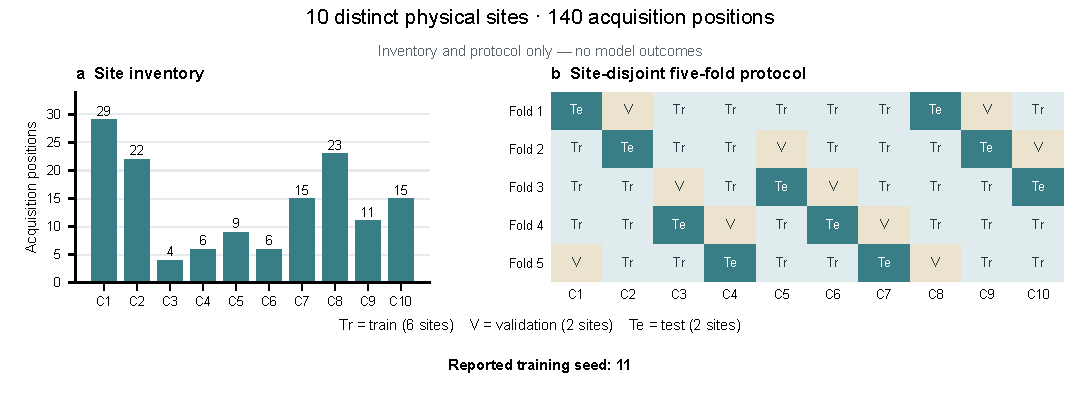
\includegraphics[width=\textwidth]{v3_inventory_folds.pdf}\caption{采集规模与当前五折协议。左图来自元数据中的真实视野数；右图为已固定划分，Tr/V/Te为训练/验证/测试。它不包含模型性能或人工精度结果。}\label{fig:inventory-folds}\end{figure}

\section{技术验证}
\subsection{当前证据状态}
现有程序提供标注读取、候选掩膜、来源贡献匹配与完整场景评价。构造输入数值验收只验证程序路径，不能当作科学性能；E5变体构建也不等于几何或任务效果验证。\pending{独立检查点残差、原始H1/H2差异、质量/内容覆盖、三池匹配统计和正式模型结果。}

计划证据包括HAV-A（六模态示例、15对残差分布、地点/视野图和H1/H2难度分层）、HAV-B（质量图集、排除面积与池可比性）和HAV-C（配对任务结果、固定位置对比）。三张配套表记录标注覆盖、精度/重复性及训练/评价支持。补充材料包含内容覆盖、缺失、空间残差、原因交集、来源贡献、指标支持、E5与受控错位。没有数值占位符被当作实验结果\cite{dodge2019,pineau2021}。

\subsection{数据池、划分与训练协议}
训练窗口为$256\times256$、stride 128并补最后起点，要求全窗口有效。未筛选池排除几何无效与隐私；筛选池进一步排除已确认的动态不一致和局部配准失败；等量随机对照逐地点等量，并只按去重覆盖面积和来源贡献匹配，不使用模型结果。实际匹配偏差与容差在评价前记录。即使候选生成成功，巡检或复核未完成也不能正式冻结。

\begin{table}[htbp]\centering\small
\caption{当前地点隔离五折协议。每地点恰好进入一次测试对；各折种子均为11、23、37、53、71。}\label{tab:protocol-zh}
\begin{tabular}{clll}\toprule 折 & 训练地点 & 验证地点 & 测试地点\\\midrule
1 & C3,C4,C5,C6,C7,C10 & C2,C9 & C1,C8\\
2 & C1,C3,C4,C6,C7,C8 & C5,C10 & C2,C9\\
3 & C1,C2,C4,C7,C8,C9 & C3,C6 & C5,C10\\
4 & C1,C2,C5,C8,C9,C10 & C4,C7 & C3,C6\\
5 & C2,C3,C5,C6,C9,C10 & C1,C8 & C4,C7\\\bottomrule\end{tabular}\end{table}

模型包括U-Net\cite{ronneberger2015unet}、pix2pix\cite{isola2017,goodfellow2014gan,mirza2014cgan}、TFD-GAN\cite{chen2026threeband,chen2026thesis}、Restormer\cite{zamir2022restormer}和pix2pix-Turbo\cite{parmar2024turbo}。归一化统计仅来自训练地点，抽样按地点平衡。预算、学习率/预热校准及验证频率尚待冻结，不使用测试集选择\cite{cawley2010}。Turbo每外循环包含两次生成器与两次判别器更新，需分别计数。先在地点内平均五种子，再地点等权汇总；配对比较使用相同地点、种子和测试支持。重叠窗口与50个地点--种子结果不构成50个独立地理样本\cite{roberts2017}。

\subsection{完整场景评价与指标支持}
所有方法和数据池条件使用共同冻结的测试支持。预测以浮点拼接，并统一截断到$[0,1]$后评价。部分指标要求邻域或矩形，其有效支持必须单独报告。
\begin{table}[htbp]\centering\small
\caption{指标定义与评价支持；这是协议，不是测量结果。}\label{tab:metrics-zh}
\begin{tabularx}{\textwidth}{p{0.19\textwidth}X}\toprule 指标 & 定义与支持\\\midrule
PSNR / MAE / RMSE\cite{huynhthu2008} & 完整场景中$[0,1]$ RGB有效配对像素，报告共同像素支持。\\
SSIM\cite{wang2004} & $11\times11$高斯窗、$\sigma=1.5$；中心的整个邻域必须有效。\\
$\Delta E_{00}$\cite{luo2001ciede2000,sharma2005} & sRGB、D65/2$^\circ$下有效像素的均值、中位数、P95；表示显示色差，不是反射率精度。\\
LPIPS\cite{zhang2018lpips} & LPIPS-Alex v0.1；预选有效矩形，实现支持边长至少64；另报矩形分数与去重覆盖面积。\\\bottomrule\end{tabularx}\end{table}

\subsection{实验范围与复用控制}
E1有125项配置，E2新增4250项多样性/数量配置；E4含2875项输入配置且已包含E1，因此E1/E2/E4共有7125项唯一配置，并非已完成的训练次数。E3外部数据（如RASMD\cite{jin2026}与EPFL可见光--近红外数据集\cite{brown2011}）需核对许可、通道和任务；未经训练的新五通道入口不能称作零样本迁移。

E5隔离六项处理：SWIR间恒等映射、既有地点级RGB标定、对启用束调整的场景关闭束调整、保留RGB辐射、羽化融合、C8--C10使用首帧RGB。各对照固定参考画布与非目标处理。原图未变时可复用原始观察；更换RGB帧后需补新帧检查点才能独立比较几何精度。受控错位在B1原生坐标定义0、0.5、1、2、4像素、四方向均衡，区分共同/单通道错位及训练/测试扰动。

\section{使用说明与局限性}
十个互异地点支持地点隔离复用，但规模较小且不是环境的代表性抽样，应报告逐地点变化和考虑依赖关系的不确定性。内容区域分数只适用于已标支持。名义通带、时分曝光、未定标数字量值与重采样共同限制光谱/空间解释。质量筛选可能提高也可能不提高模型指标，阴性结果与残余匹配偏差均应保留。独立人工证据、任务效用和公开复现相互补充，不能互相替代。

\section*{代码可用性}
作者已有本地处理与评价实现。\pending{公开代码链接、固定提交、依赖、许可及投稿前的独立最小复现核查。}
\section*{数据可用性声明}
拟使用Zenodo与CC BY 4.0数据许可，需作者核实发布权利和范围。\pending{最终版本、DOI、数据引用、匿名审稿链接、隐私审查与下载哈希验证。}

\pending{以下作者贡献、资助和利益冲突沿用原稿，需全体作者最终核对。}
\section*{作者贡献}
杜虎：概念构思、数据整理、形式分析、调查研究、方法设计、软件实现、验证、可视化和初稿撰写。刘晓：概念构思、方法设计、项目管理、资源提供、指导、验证和稿件审阅与修改。杜丽丽：数据整理、调查研究、资源提供、验证和稿件审阅与修改。宋波：调查研究、资源提供、验证和稿件审阅与修改。孙晓兵：概念构思、项目管理、资源提供、指导和稿件审阅与修改。

\section*{基金项目}
本 Data Descriptor 的整理与撰写未获得新增专项经费资助。

\section*{利益冲突}
作者声明不存在竞争性利益。

\bibliographystyle{unsrtnat}
\bibliography{refs}
\end{document}
